\documentclass[a4paper,10pt]{report}
\usepackage[utf8]{inputenc}

% Title Page
\author{Łukasz Adamowicz}

\usepackage{mathcommands}
\usepackage{amsthm}
\usepackage{algorithm}
\usepackage{algpseudocode}
\usepackage{hyperref}
\usepackage{graphicx}
\usepackage{float}
\newtheorem{theorem}{Theorem}
\newtheorem{statement}{Statement}
\newtheorem{lemma}{Lemma}
\newtheorem{remark}{Remark}
\renewcommand{\thesection}{\arabic{section}}
\begin{document}
% \maketitle
\begin{titlepage}
    \begin{center}
        \textbf{\Large Fine-tuning STRUCTURES25 model with implicit loss}\\[2cm]
        \textbf{Academic Year:} 2024--2025\\
        \textbf{Master's Program:} M2 Mathématiques, Modélisation et Apprentissage\\
        \textbf{Name:} Łukasz Adamowicz\\[1cm]
        \textbf{Internship Supervisor:} Professor Fred Hamprecht\\
        \textbf{Email:} fred.hamprecht@iwr.uni-heidelberg.de\\[1cm]
        \textbf{Hosting institution:}\\
        Heidelberg University,\\
        Interdisciplinary Center for Scientific Computing\\
        \textbf{UFR Contact:}\\
        Alexis Glaunes\\
        alexis.glaunes@parisdescartes.fr\\[2cm]

        % Optionally add logos, date, etc.
        \vfill
        \today
    \end{center}
\end{titlepage}


\begin{abstract}

During my internship at Hamprecht Lab, an investigation was conducted on fine-tuning deep learning models using a loss function defined in an implicit way.

The goal of the internship was to adapt and implement the approach from the preprint \cite{neuralscf} to a setting used in Hamprecht lab.

Two approaches to gradient computation were implemented: equilibrium propagation and jacobian approach. A stability issue arose, but was subsequently resolved. The results showed that the equilibrium propagation approach might be viable, whereas the jacobian approach did not work at all.
\end{abstract}


\tableofcontents
\newpage
\section{Lab presentation}


%  Since $E(\theta, p)$ is a approximation of physical potential, it's reasonable to assume that hessian is positive-definite at the minimum.

The current focus of the ScientificAI group is on applying deep learning to orbital-free density functional theory (OF-DFT).

 To accurately predict molecular properties, quantum mechanics formalism can be employed to solve for the electronic structure, but for big molecules this approach is not tractable.

However a theorem by Hohenberg-Kohn has shown that all that's needed to know the electronic structure is the ground state electron density $\rho_{gs}$ and that there exists an energy functional such that
\begin{equation}
 \rho_{gs} = \argmin_\rho E[\rho].
\end{equation}


Exact form of the energy functional $E[\rho]$ remains unknown. The goal of  project is to approximate the energy functional $E[\rho]$ using a deep learning model (a surrogate functional) denoted as $E(\theta, \rho)$.

If successful, this would enable the computation of the ground-state electron density with a complexity of $O(n)$, thereby allowing for efficient simulations of large molecules. Since the exact ground state is not always known, the model must be capable of converging from a wide range of initial starting points.

The electron density $\rho(\vec{r})$ is approximated as a linear combination of atom-centered smooth functions $\omega_i$, that is:

\[
\rho(\vec{r}) = \sum_{i=1}^n p_i \omega_i(\vec{r})
\]

The specific number and type of functions $\omega_i$ depend on the atoms in the system.

The integral of the electron density yields the total number of electrons in the system:

\[
N = \int_{\mathbb{R}^3} \rho(\vec{r}) d\vec{r} = \sum_{i=1}^n p_i \int_{\mathbb{R}^3} \omega_i(\vec{r}) d\vec{r}.
\]

By defining a vector $w = (w_1, \ldots, w_n)$ where each component is:

\[
w_i = \int_{\mathbb{R}^3} \omega_i(\vec{r}) d\vec{r},
\]

we can express the total electron count as:

\[
\langle w, p \rangle = N.
\]



\newpage

\section{Theory part}
Notation: Let $E(\theta, M ,p)$ denote the energy model, with $\theta \in \R^k$ being model parameters, $M$ the molecule information, and $p=(p_1, \ldots ,p_n )\in \R^n$ electron density coefficients.  We assume that $E(\theta, M ,p)$ is smooth with respect to $\theta$ and $p$.
By $\frac{d}{d\theta}$ we mean total derivative, while $\pd{}{\theta}$ denotes partial derivative $\theta$, when all other arguments are held constant. Then $\pd{E}{p}$ is a row vector of size $n$, hessian $\frac{\partial^2 E}{ \partial p^2 }$ is a matrix of size $n \times n$, and $\frac{\partial^2 E}{\partial \theta \partial p}$ is a matrix of size $n \times k $.


\subsection{Goal of the project}
The goal of the project was to investigate and minimize the following loss
\begin{equation}\label{bilevel}
 \min_\theta \sum_i \mathcal{L}(p_{\theta}^{M_i}),
\end{equation}
where
\begin{equation}
  p_\theta^{M_i}:=\argmin_{p : \inner{w}{p}=N_i} E(\theta,M_i,p)
\end{equation}
and $\mathcal{L}_{M_i}(p) = \frac{1}{2}\mse{p-p_{M_i}}$ is the standard $L_2$ loss.

In the rest of the report I will drop index $M_i$. The reason is it will simplify the notation significantly, while not impacting the gradient derivation in any notable way.
Therefore I will write $E(\theta,p)$ instead of $E(\theta,M,p)$ and the same for $p_\theta$, $\mathcal{L}(p)$ and so on.
The quantity $\pth$ is a \textbf{fixed point}.
This optimization problem falls under the domain of \textbf{bilevel optimization}.

The main problem lies in computing the gradient of $\mathcal{L}(p_\theta)$ and it will be the main subject of this report.

\begin{remark}[Motivating the loss function] Finding a ground state electron density of a molecule is a fundamental problem in quantum chemistry. Usual methods are too computationally expensive for big systems. Surrogate functionals are used to approximate true energy functional and through that approximate the ground state by computing fixed point of the surrogate functional. In that light, minimizing the error between ground state density and fixed point of the model makes a certain amount of sense.
\end{remark}



\subsubsection{One molecule}
Let $w$ be a non-zero vector and $N>0$ a positive number.
We consider the problem of minimizing

\begin{equation}
 \min_\theta \mathcal{L}(p_\theta),
\end{equation}
with
\begin{equation}
\pth = \argmin_{\substack{p \in \R^n \\ p: \inner{p}{w}=N }} E(\theta, p)
\end{equation}
and
\begin{equation}
 \mathcal{L}(p) = \frac{1}{2} \norm{p-p_{gs}}^2,
\end{equation}
where $p_{gs}$ are ground state density coefficients given by the data and satisfy the constraint $\inner{p_{gs}}{w} = N$.


\subsubsection{Direct approach to gradient computation}
The most direct approach would be to backpropagate through the trajectory of the fixed point. More precisely, we run gradient descent and obtain a trajectory $p_1, \ldots, p_T$, where $p_T \approx \pth$. We can store this trajectory in memory and use backpropagation on the loss
\begin{equation}
 \mathcal{L}(p_T(\theta)) \approx \mathcal{L}(\pth)
\end{equation}
Although straightforward there are a few issues with this approach.
\begin{itemize}
 \item backpropagation through the whole trajectory is very memory intensive, therefore fixed point search can be run for very low number of steps.
 \item the gradient depends on the starting point
 \item can't apply warm-starting to speed up the training. In theory, for jacobian and equilibrium propagation approach we can find the fixed point once and reuse it in subsequent runs as a starting point, therefore making training much faster.
 However, due to stability issues and difficulties of tracking loss, I ended up not using warm-starting.
\end{itemize}


\subsection{Implicit function theorem}
This can be accomplished by using implicit function theorem. In the rest of the document I will refer to computation of the gradient using this method as \textbf{jacobian approach}.

I use the version of implicit function theorem from \cite{zucchet2022beyond}, which in turn is taken from \cite{dontchev2009implicit}.
\begin{theorem}[Implicit Function Theorem, \cite{zucchet2022beyond} ]
Let $G(\theta, p): \R^k \times \R^n \to \R^n$ be $C^1$ and $(\bar{\theta}, \bar{p})$ such that $G(\bar{\theta},\bar{p})=0$. If the jacobian
$\pd{G}{p}(\bar{\theta},\bar{p})$ is non-singular, then there exists an open neighbourhood $U$ of $\bar{\theta} $ and a function $p(\theta):U \to \R^n$, such that $G(\theta, p(\theta)) = 0$ and $p(\bar{\theta}) = \bar{p}$. Moreover, $p(\theta)$ is also differentiable with
its derivative given by
\begin{equation}
\pd{p(\theta)}{\theta}= - \bigg(\pd{G}{p}(\theta, p(\theta))\bigg)^{-1} \frac{\partial^2 G}{\partial \theta \partial p}(\theta, p(\theta)).
\end{equation}

\end{theorem}
In our case $G = \pd{E}{p}$. Since our model is $C^1$/smooth with respect to its arguments and the hessian of $E$ is assummed to be positive definite, the conditions of the theorem are satisfied.


\subsubsection{Basis-dependent approach}

First, let's consider the problem in an orthogonal basis containing $w$. Let the basis be $(e_1,\ldots, e_{n-1}, w)$. Define $\widetilde{E}(\theta, p) = E(\theta, p_{gs}+ p)$ and $p = \sum_{i=1}^{n-1} p_i e_i$. Then $\widetilde E(\theta, \cdot)$ is just $E$ restricted to the affine space $p_{gs}+\text{span}(w)^\perp$, and the problem becomes

\begin{equation}
  \min_\theta \mathcal{L}(p_\theta),
\end{equation}

\begin{equation}
 p_\theta = \argmin_{p\in \R^{n-1}} \widetilde{E}(\theta, p)
\end{equation}

We will find the gradient with the help of the implicit function theorem.

\begin{statement}
The gradient of $\mathcal{L}(p_\theta)$ is equal to
 \begin{equation}
 \frac{\partial \mathcal{L}(p_\theta)}{\partial \theta} = -(\pth - p_{gs}) \bigg(\frac{\partial^2  \widetilde{E}}{\partial p^2}\bigg)^{-1}  \frac{\partial^2  \widetilde{E}}{\partial \theta \partial p}
\end{equation}
\end{statement}

To obtain the gradient of the loss, we start from the chain rule
\begin{equation}
 \frac{\partial \mathcal{L}(p_\theta)}{\partial \theta} = \frac{\partial \mathcal{L}}{\partial p}\frac{\partial p_\theta}{\partial \theta}.
\end{equation}

Since $\frac{\partial \mathcal{L}}{\partial p}(p_\theta)= p_\theta-p_{gs}$, all we need to find is $\frac{\partial p_\theta}{\partial \theta}.$

\begin{statement}
The gradient of $p_\theta$ is equal to
 \begin{equation}
   \frac{\partial p_\theta}{\partial \theta} = -\bigg(\frac{\partial^2 \widetilde{E}}{\partial p^2}\bigg)^{-1} \frac{\partial^2 \widetilde{E}}{\partial \theta \partial p}(\theta, p_\theta)
 \end{equation}
\end{statement}

\begin{proof}
By definition, $\widetilde{E}(\theta, \cdot)$ attains its minimum at $p_\theta$, so it follows that
\begin{equation}
\frac{\partial \widetilde{E}}{\partial p}(\theta, p_\theta) = 0.
\end{equation}

By taking derivative with respect to $\theta$, we get

% total derivative
\begin{equation}
0=\frac{\partial}{\partial \theta}\left(\frac{\partial \widetilde{E}}{\partial p}(\theta, p_\theta)\right) = \frac{\partial^2 \widetilde{E}}{\partial \theta \partial p} + \frac{\partial^2 \widetilde{E}}{\partial p^2} \frac{\partial p_\theta}{\partial \theta}.
\end{equation}
Therefore
\begin{equation}
 \frac{\partial p_\theta}{\partial \theta} = -\left(\frac{\partial^2 \widetilde{E}}{\partial p^2}\right)^{-1} \frac{\partial^2 \widetilde{E}}{\partial \theta \partial p}(\theta, p_\theta).
\end{equation}

Let's denote the Hessian of $\widetilde{E}$ as

\begin{equation}
H := \frac{\partial^2 \widetilde{E}}{\partial p^2}(\theta,p_\theta)
\end{equation}
\end{proof}
This gives us the final formula
\begin{equation}
 \frac{\partial}{\partial \theta}\mathcal{L}(p_\theta) = - (p_\theta - p_{gs}) H^{-1}  \left.\frac{\partial^2 \widetilde{E}}{\partial \theta \partial p}\right|_{p=p_\theta, \theta=\theta}.
\end{equation}

\subsubsection{Basis-free approach}
Let's reformulate the problem without relying on a specific basis.
We want to find
\begin{equation}
 \min_\theta \mathcal{L}(p_\theta),
\end{equation}
with
\begin{equation}
p_\theta = \argmin_{\substack{p \in \R^n \\ p: \langle p, w\rangle=N }} E(\theta, p).
\end{equation}


 To this end we make use of the following lemma.

\begin{lemma}
 Let $P := I -\frac{ww^T}{w^Tw} $ be the projection operator onto subspace $V = \text{span}(w)^{\perp}$. Then the following equality is true
 \begin{equation}
  P\left(\pd{E}{p}(\theta, p_\theta)\right) = 0
 \end{equation}

\end{lemma}
\begin{proof}
  Since $p_\theta$ is the minimum of $E(\theta,p)$ restricted to $V+p_{gs}$ we have \[\langle \pd{E}{p}(\theta,p_{\theta}), u \rangle = 0\] for any $u\in V$. Taking $u = P\big( \pd{E}{p}(\theta,p_\theta)\big)$ we obtain
  \[\langle \pd{E}{p}(\theta,p_{\theta}), P\big( \pd{E}{p}(\theta,p_\theta)\big) \rangle = \norm{P\big( \pd{E}{p}(\theta,p_\theta)\big)}^2=0,\]
  which concludes the proof.
\end{proof}

Let's denote $F(\theta,p) :=P \left(\pd{E}{p}(\theta,p)\right).$ Then the previous condition can be written as
\begin{equation}
 F(\theta,p_\theta) = 0.
\end{equation}
We take the derivative with respect to $\theta$
\begin{equation}
0=\dth{F(\theta, p_\theta)} = \pd{F}{\theta}(\theta,p_\theta) + \pd{F}{p}(\theta,p_\theta) \dth{p_\theta}.
\end{equation}
Rearranging we obtain
\begin{equation}
 \frac{d p_\theta}{d\theta} = - \bigg(\pd{F}{p}(\theta,p_\theta)\bigg)^{-1} \pd{F}{\theta}(\theta,p_\theta).
\end{equation}

Therefore the full gradient of $\mathcal{L}(p_\theta)$ is equal to
\begin{equation}
 \dth{\mathcal{L}(p_\theta)} = - (p_\theta - p_{gs})\bigg(\pd{F}{p}(\theta,p_\theta)\bigg)^{-1} \pd{F}{\theta}(\theta,p_\theta).
\end{equation}
 \begin{remark}
 The jacobian $\pd{F}{p}$ is not invertible, since $F$ is a projection.
  \begin{equation}
   F(\theta, p) = \sum_{i=1}^{n-1} \inner{\pd{E}{p}(\theta, p)}{e_i} e_i +  0 \cdot w
  \end{equation}
%
 The jacobian matrix in the basis $(e_0,...,e_{n-1},w)$ can be written as \begin{equation}
                      \frac{\partial F}{\partial p}\bigg|_{p=\pth} =\begin{bmatrix}
H & 0 \\
0 & 0
\end{bmatrix}.
\end{equation}

and solution to linear regression
\begin{equation}
 y = \underset{u\in \R^n}{\mathrm{argmin }}\bigg\|u \begin{bmatrix}
H & 0 \\
0 & 0
\end{bmatrix} + (p_\theta-p_{true})\bigg\|^2
\end{equation}
is satisfied for by $y$ of the form

\begin{equation}
 y = P\big((\pth-p_{gs})\big)H^{-1} + \alpha w.
\end{equation}
Since $F$ is a projection onto plane perpendicular to $w$, it shouldn't matter which $y$ we choose.
That is to say
\begin{equation}
 \inner{y}{ \pd{F}{\theta}}=\inner{Py}{\pd{F}{\theta}}.
\end{equation}



Therefore, the formula doesn't change, however some algorithms for solving linear systems might not work, if they rely on invertibility.

\end{remark}
In the rest of the report I will reference the procedure of finding $y$ vector as \textbf{solving the linear equation}.


We can rewrite the formula for the gradient as
\begin{equation}
 \dth{\mathcal{L}(\pth)} = y \cdot  \frac{\partial F}{\partial \theta}\bigg|_{p=p_\theta, \theta=\theta}
\end{equation}

treat $y$ as constant vector and pull it inside partial derivative to obtain

\begin{equation}
 \dth{\mathcal{L}(\pth)} =   \frac{\partial (\inner{y}{F})}{\partial \theta}\bigg|_{p=p_\theta, \theta=\theta}.
\end{equation}

% To make $y$ unique we add a term such as $\inner{u}{w}^2$ or add additional constraints.


The whole procedure for gradient calculation is as below
\begin{algorithm}[H]
\caption{Jacobian approach gradient Calculation}
\begin{algorithmic}[1]
\Require Data $p_{gs}$, model parameters $\theta$
\State  Solve for $p_\theta  = \argmin_{\substack{p \in \R^n \\ p: \inner{p}{w}=N }} E(\theta, p).$
\State Solve for $y = \underset{u\in \mathbb{R}^n}{\mathrm{argmin}} \bigg\|u \frac{\partial F}{\partial p}\bigg|_{p=p_\theta} + (p_\theta-p_{gs})\bigg\|^2$
\State Compute gradient $\dth{\mathcal{L}(\pth)} = \frac{\partial (\inner{y}{F})}{\partial \theta}\bigg|_{\substack{p=p_\theta \\\theta= \theta}}$
\State \Return $\dth{\mathcal{L}(\pth)}$
\end{algorithmic}
\end{algorithm}


The quantity $\frac{\partial (\inner{y}{F})}{\partial \theta}\bigg|_{\substack{p=p_\theta \\\theta= \theta}}$ can be obtained using automatic differentation.  Similarly $u \frac{\partial F}{\partial p}\bigg|_{p=p_\theta}$ can be computed with automatic differentation and without storing the full jacobian matrix in memory. This matters for bigger batch sizes and molecules, since the memory cost scales quadratically. Matrix-free methods were used to solve for $y$ vector.


The implementation details, such as root-solver, are described in \ref{sec:impl}.

\subsection{Jacobian approach experiments and results}

\subsubsection{Convergence thresholds}
 I tested the algorithm with various tolerance threshold and training learning rate on both fixed point search and linear equation solver.
I found out that strict thresholds on fixed point search hindered training completely. The loss increased during training and varying both learning rate and the tolerance on linear equation solving did not change this fact. Even when the loss decreased at first it could increase later as shown in Figure~\ref{fig:jac-eqprop-loss}.


\begin{figure}[h!]
 \centering
 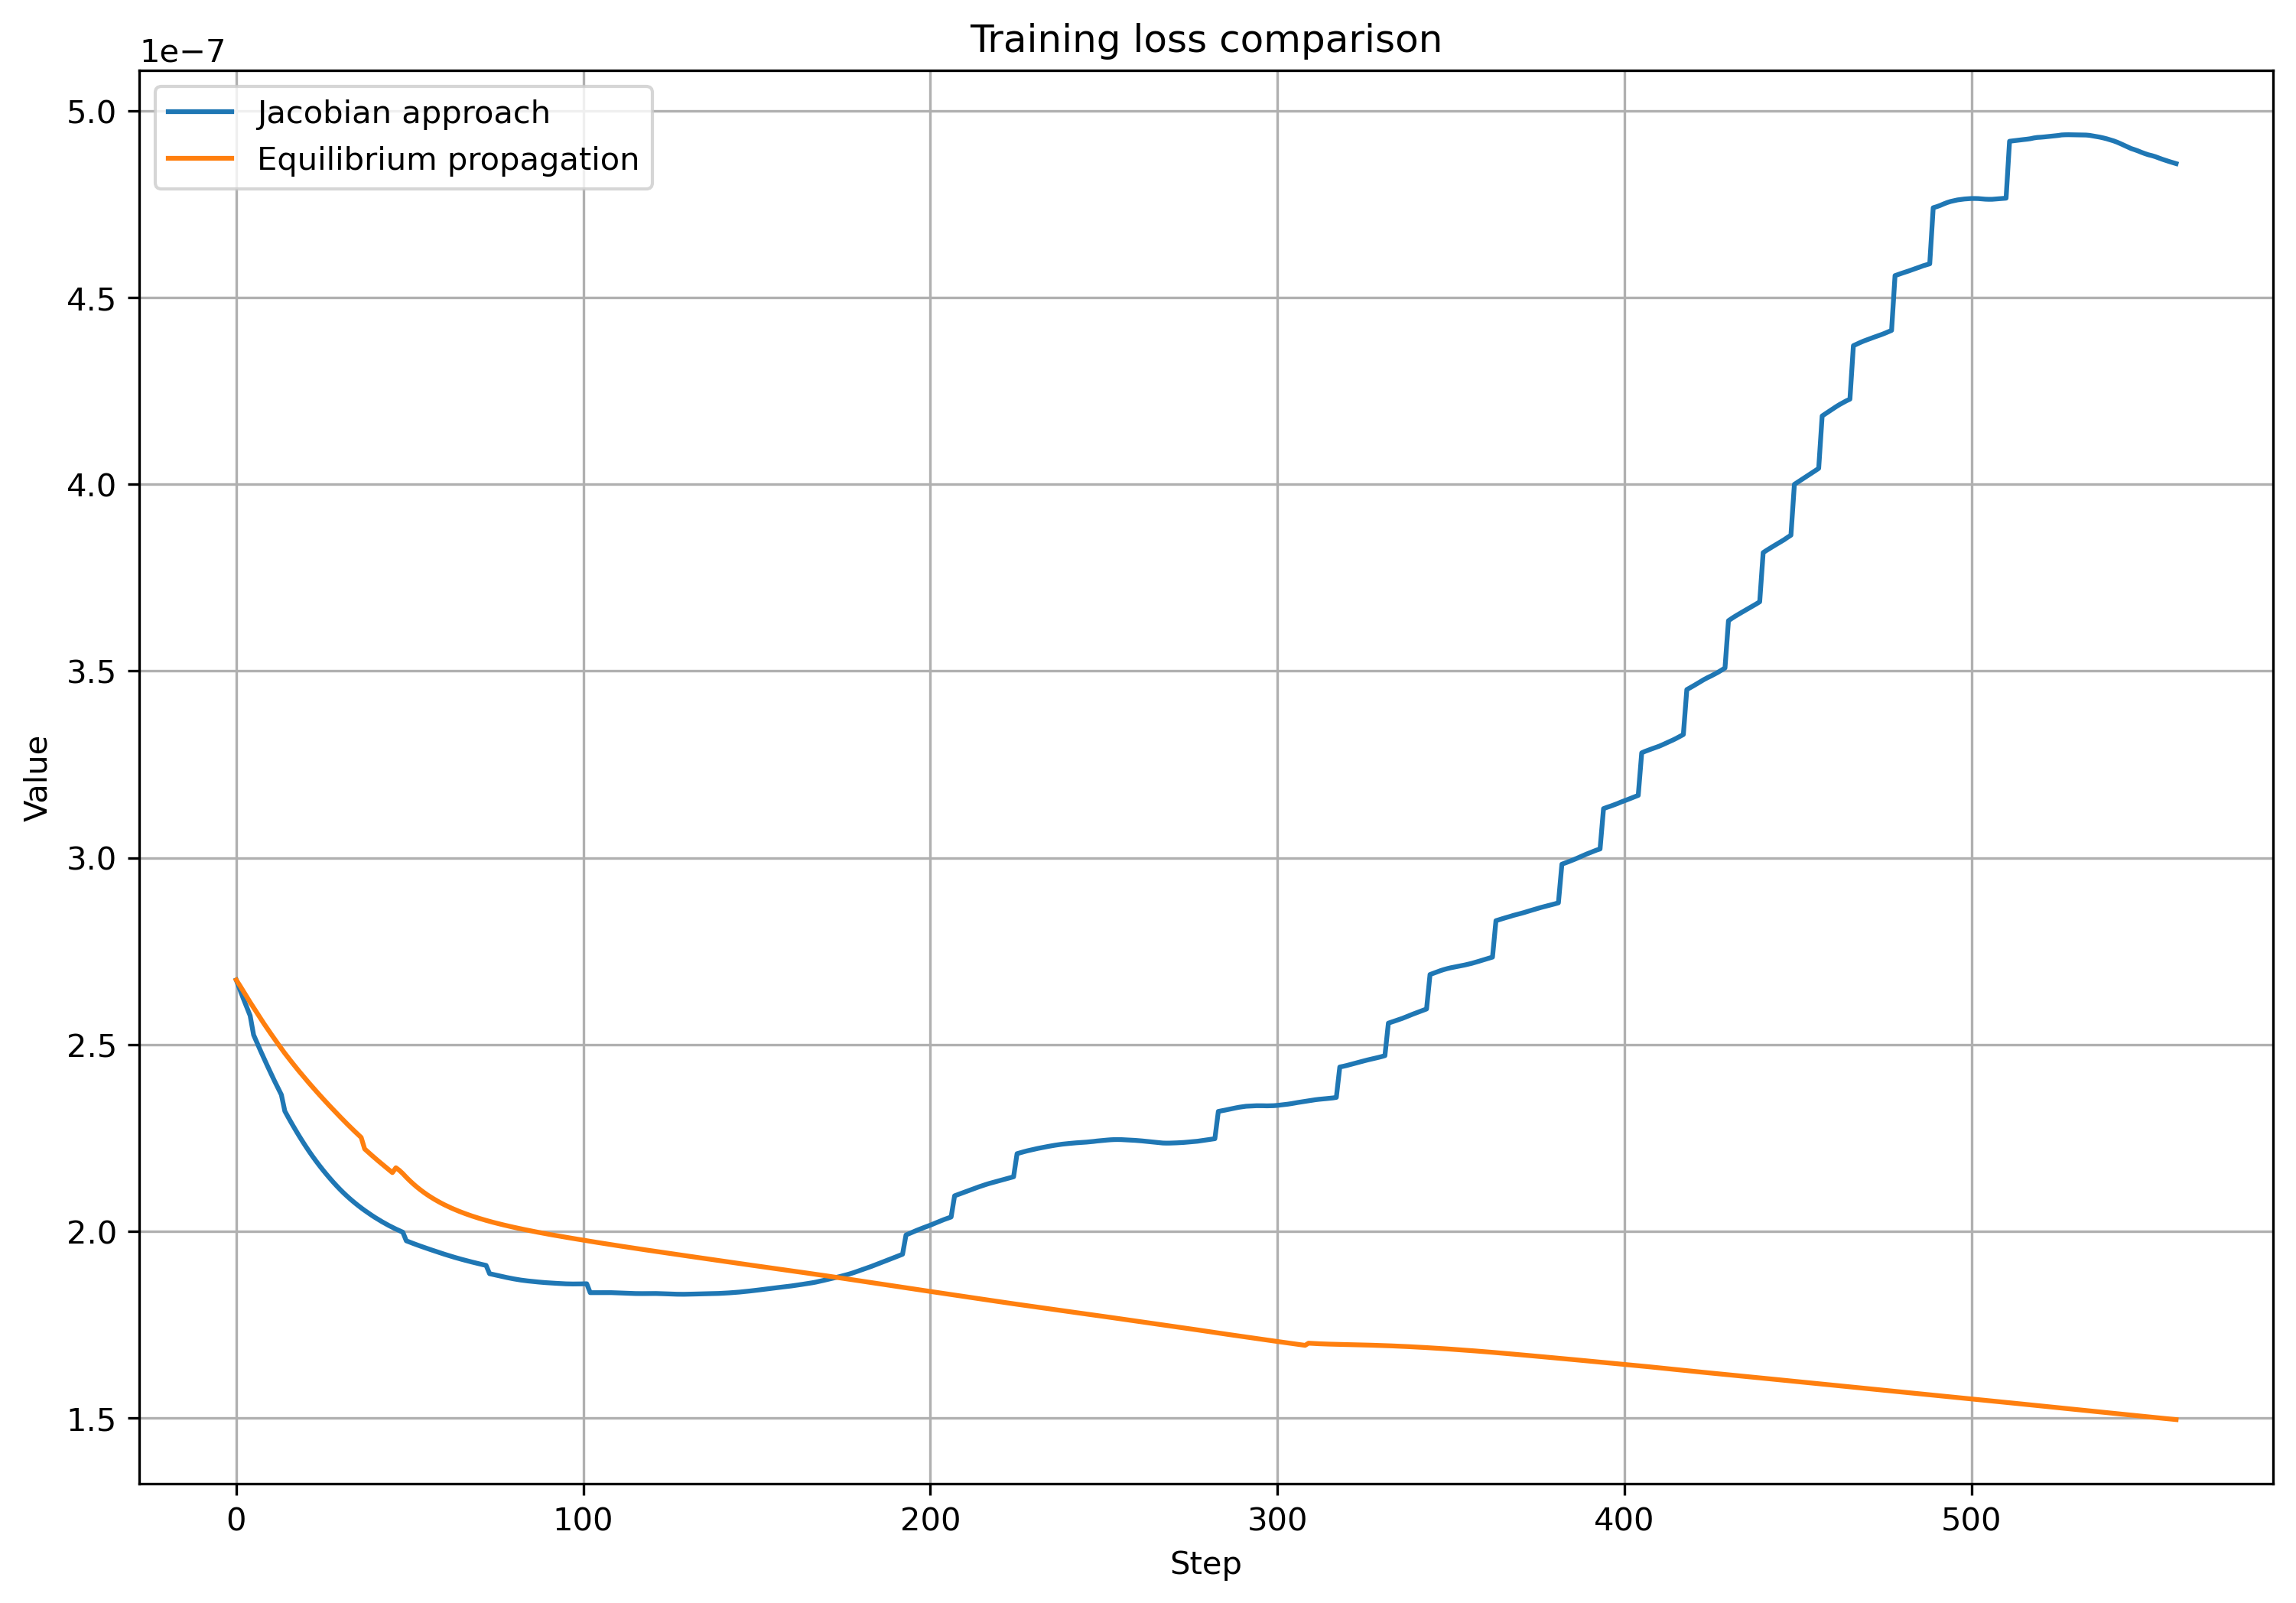
\includegraphics[scale=0.5]{images/loss_comparison.png}
 \caption{Comparison of training loss for jacobian and EP approaches. Jacobian approach decreases loss at first, but starts diverging later. Equilibrium propagation seems to be more stable.}
 % loss_comparison.png: 3002x2096 px, 300dpi, 25.42x17.75 cm, bb=0 0 720 50
 \label{fig:jac-eqprop-loss}
\end{figure}



TK DENOP PICTURES

\subsubsection{Conjugate gradient}
I implemented and tested conjugate gradient method for solving linear system. However, the algorithm rapidly diverged and proved to be unsuitable.
\subsubsection{Summary of jacobian appraoch}

 For reasons yet unknown to me I have not been able to make jacobian approach work for the purpose of finetuning the model. Despite loss function decreasing during course of the training, density difference during density optimization run did not improve. This suggests, that jacobian approach did not in fact move the fixed point $\pth$ to real ground state $p_{gs}$ or did it while making energy landscape much more difficult to navigate.


\subsection{ Equilibrium propagation}

\subsubsection{Base version}
During my internship I also implemented and tested optimization using Equilibrium Propagation (see \cite{eqprop}, \cite{zucchet2022beyond}), which is an alternative method of computing the gradient with respect to model parameters.
Let's denote
\begin{equation}
H(\theta, p, \beta) := \beta \mathcal{L}(p) + E(\theta, p),
\end{equation}
where $\beta \in \R$.
 This is called \textbf{total energy} in \cite{eqprop}. Let's also denote
\begin{equation}
p_{\theta}^{\beta}:=\argmin_p H(\theta, p, \beta)
\end{equation}
\begin{remark}
 For $\beta>0$ the function $p \mapsto \beta \mathcal{L}(p)$ is strongly convex, so $H$ has ... TK HOW TO WRITE should converge better
 \end{remark}
 \begin{remark}
   Since $H(\theta,p,0) = E(\theta,p)$ we have $p_{\theta}^{0}=p_{\theta}$.
 \end{remark}







\begin{statement}[Equilibrium propagation formula]
 \begin{equation}
 \frac{d}{d\theta} \mathcal{L}(p_\theta) = \lim_{\beta \to 0} \frac{\pd{H}{\theta}(\theta, p_\theta^\beta, \beta)-\pd{H}{\theta}(\theta, p_\theta^0, 0) }{\beta} = \lim_{\beta \to 0}\frac{1}{\beta} \pd{}{\theta} \bigg(H(\theta, p_\theta^\beta,\beta) - H(\theta, p_\theta^0, 0)\bigg).
\end{equation}
\end{statement}
\begin{remark}

This formula can be used to numerically approximate the gradient of the loss function.
Since in our case $\mathcal{L}(p)$ doesn't depend on $\theta$, $\pd{H}{\theta}$ simplifies to $\pd{E}{\theta}$, although the formula remains true, when $\mathcal{L}$ is also a function of $\theta$. For example there might be regularization term added to $\mathcal{L}(p)$.
\end{remark}


\begin{proof} Let's denote
 \begin{equation}
 G(\theta, \beta) := H(\theta, p_\theta^\beta, \beta).
\end{equation}
Because $p_\theta^\beta$ is $C^2$, $G$ is $C^2$ and so we have the symmetry of second derivatives
\begin{equation}
 \frac{d}{d\theta}\frac{d}{d\beta}G(\theta,\beta)\big|_{\beta=0, \theta = \theta} =\frac{d}{d\beta}\frac{d}{d\theta}G(\theta,\beta)\big|_{\beta=0, \theta = \theta}
\end{equation}
We have

\begin{equation}\label{eqcond}
 \frac{dG}{d\beta} = \frac{\partial H}{\partial \beta} + \frac{\partial H}{\partial p}(\theta,\pthb, \beta)\frac{\partial \pthb}{\partial \beta}.
\end{equation}
By definition
\begin{equation}
\frac{\partial H}{\partial p}(\theta,\pthb, \beta)=0.
\end{equation}
The second term vanishes, leaving us with
\begin{equation}\label{pvanish}
  \frac{dG}{d\beta}\big|_{\beta=0} = \frac{\partial H}{\partial \beta}(\theta, \pth, 0)=\mathcal{L}(\pth).
\end{equation}
Analogically
\begin{equation}\label{thvanish}
 \frac{dG}{d\theta}=\frac{\partial H}{\partial \theta}(\theta, \pthb, \beta).
\end{equation}

TK Explain, why it's different iwe we switch back the order of derivatives.
In the end we obtain
\begin{align}
 \frac{d}{d\theta} \mathcal{L}(p_\theta) &=\frac{d}{d\theta}\frac{d}{d\beta}G(\theta,\beta)\big|_{\beta=0} = \frac{d}{d\beta}\frac{d}{d\theta}G(\theta,\beta)\big|_{\beta=0}=\\
 &=\lim_{\beta \to 0}\frac{1}{\beta} \pd{}{\theta} \bigg(H(\theta, p_\theta^\beta,\beta) - H(\theta, p_\theta^0, 0)\bigg)
\end{align}

\end{proof}

\begin{remark}
 It turns out the formula remains the same if we change the fixed point definition to
\begin{equation}
 p_\theta^\beta = \argmin_{\substack{p \in \R^n \\ p: \inner{p}{w}=N }} H(\theta, p, \beta)
\end{equation}
In this case equilibrium condition \ref{eqcond} changes to
\begin{equation*}
P\bigg(\frac{\partial H}{\partial p}(\theta,\pthb, \beta)\bigg)=0,
\end{equation*}
where, as before, $P$ is a projection operator. Since $\inner{w}{\pthb}$ is does not depend on $\beta$ nor $\theta$ both \ref{pvanish} and \ref{thvanish} also stay the same and so the final formula remains unchanged.

\end{remark}



\begin{algorithm}[H]
\caption{Equilibrium propagation algorithm}
\begin{algorithmic}[1]
\Require Data $p_{gs}$, model parameters $\theta$, $\beta>0$.
\State  Solve for $p_\theta^0  = \argmin_{\substack{p \in \R^n \\ p: \inner{p}{w}=N }} H(\theta, p, 0).$
\State Solve for $p_\theta^\beta  = \argmin_{\substack{p \in \R^n \\ p: \inner{p}{w}=N }} H(\theta, p, \beta).$
\State Compute gradient $\dth{\mathcal{L}(\pth)} = \frac{1}{\beta} \pd{}{\theta} \bigg(H(\theta, p_\theta^\beta,\beta) - H(\theta, p_\theta^0, 0)\bigg)$
\State \Return $\dth{\mathcal{L}(\pth)}$
\end{algorithmic}
\end{algorithm}


\subsection{Equilibrium propagation experiments}
In contrast to jacobian approach I managed to finetune the model on single molecule.
The training loss decreased. What is much more important is that density difference also decreased, when fixed point search was run from a different starting point.
TK DENOP FOR EQPROP
\subsubsection{Varying $\beta$ parameter}
I tested equilibrium propagation for different values of parameter $\beta$.

TK conclusions
\begin{figure}[H]
 \centering
 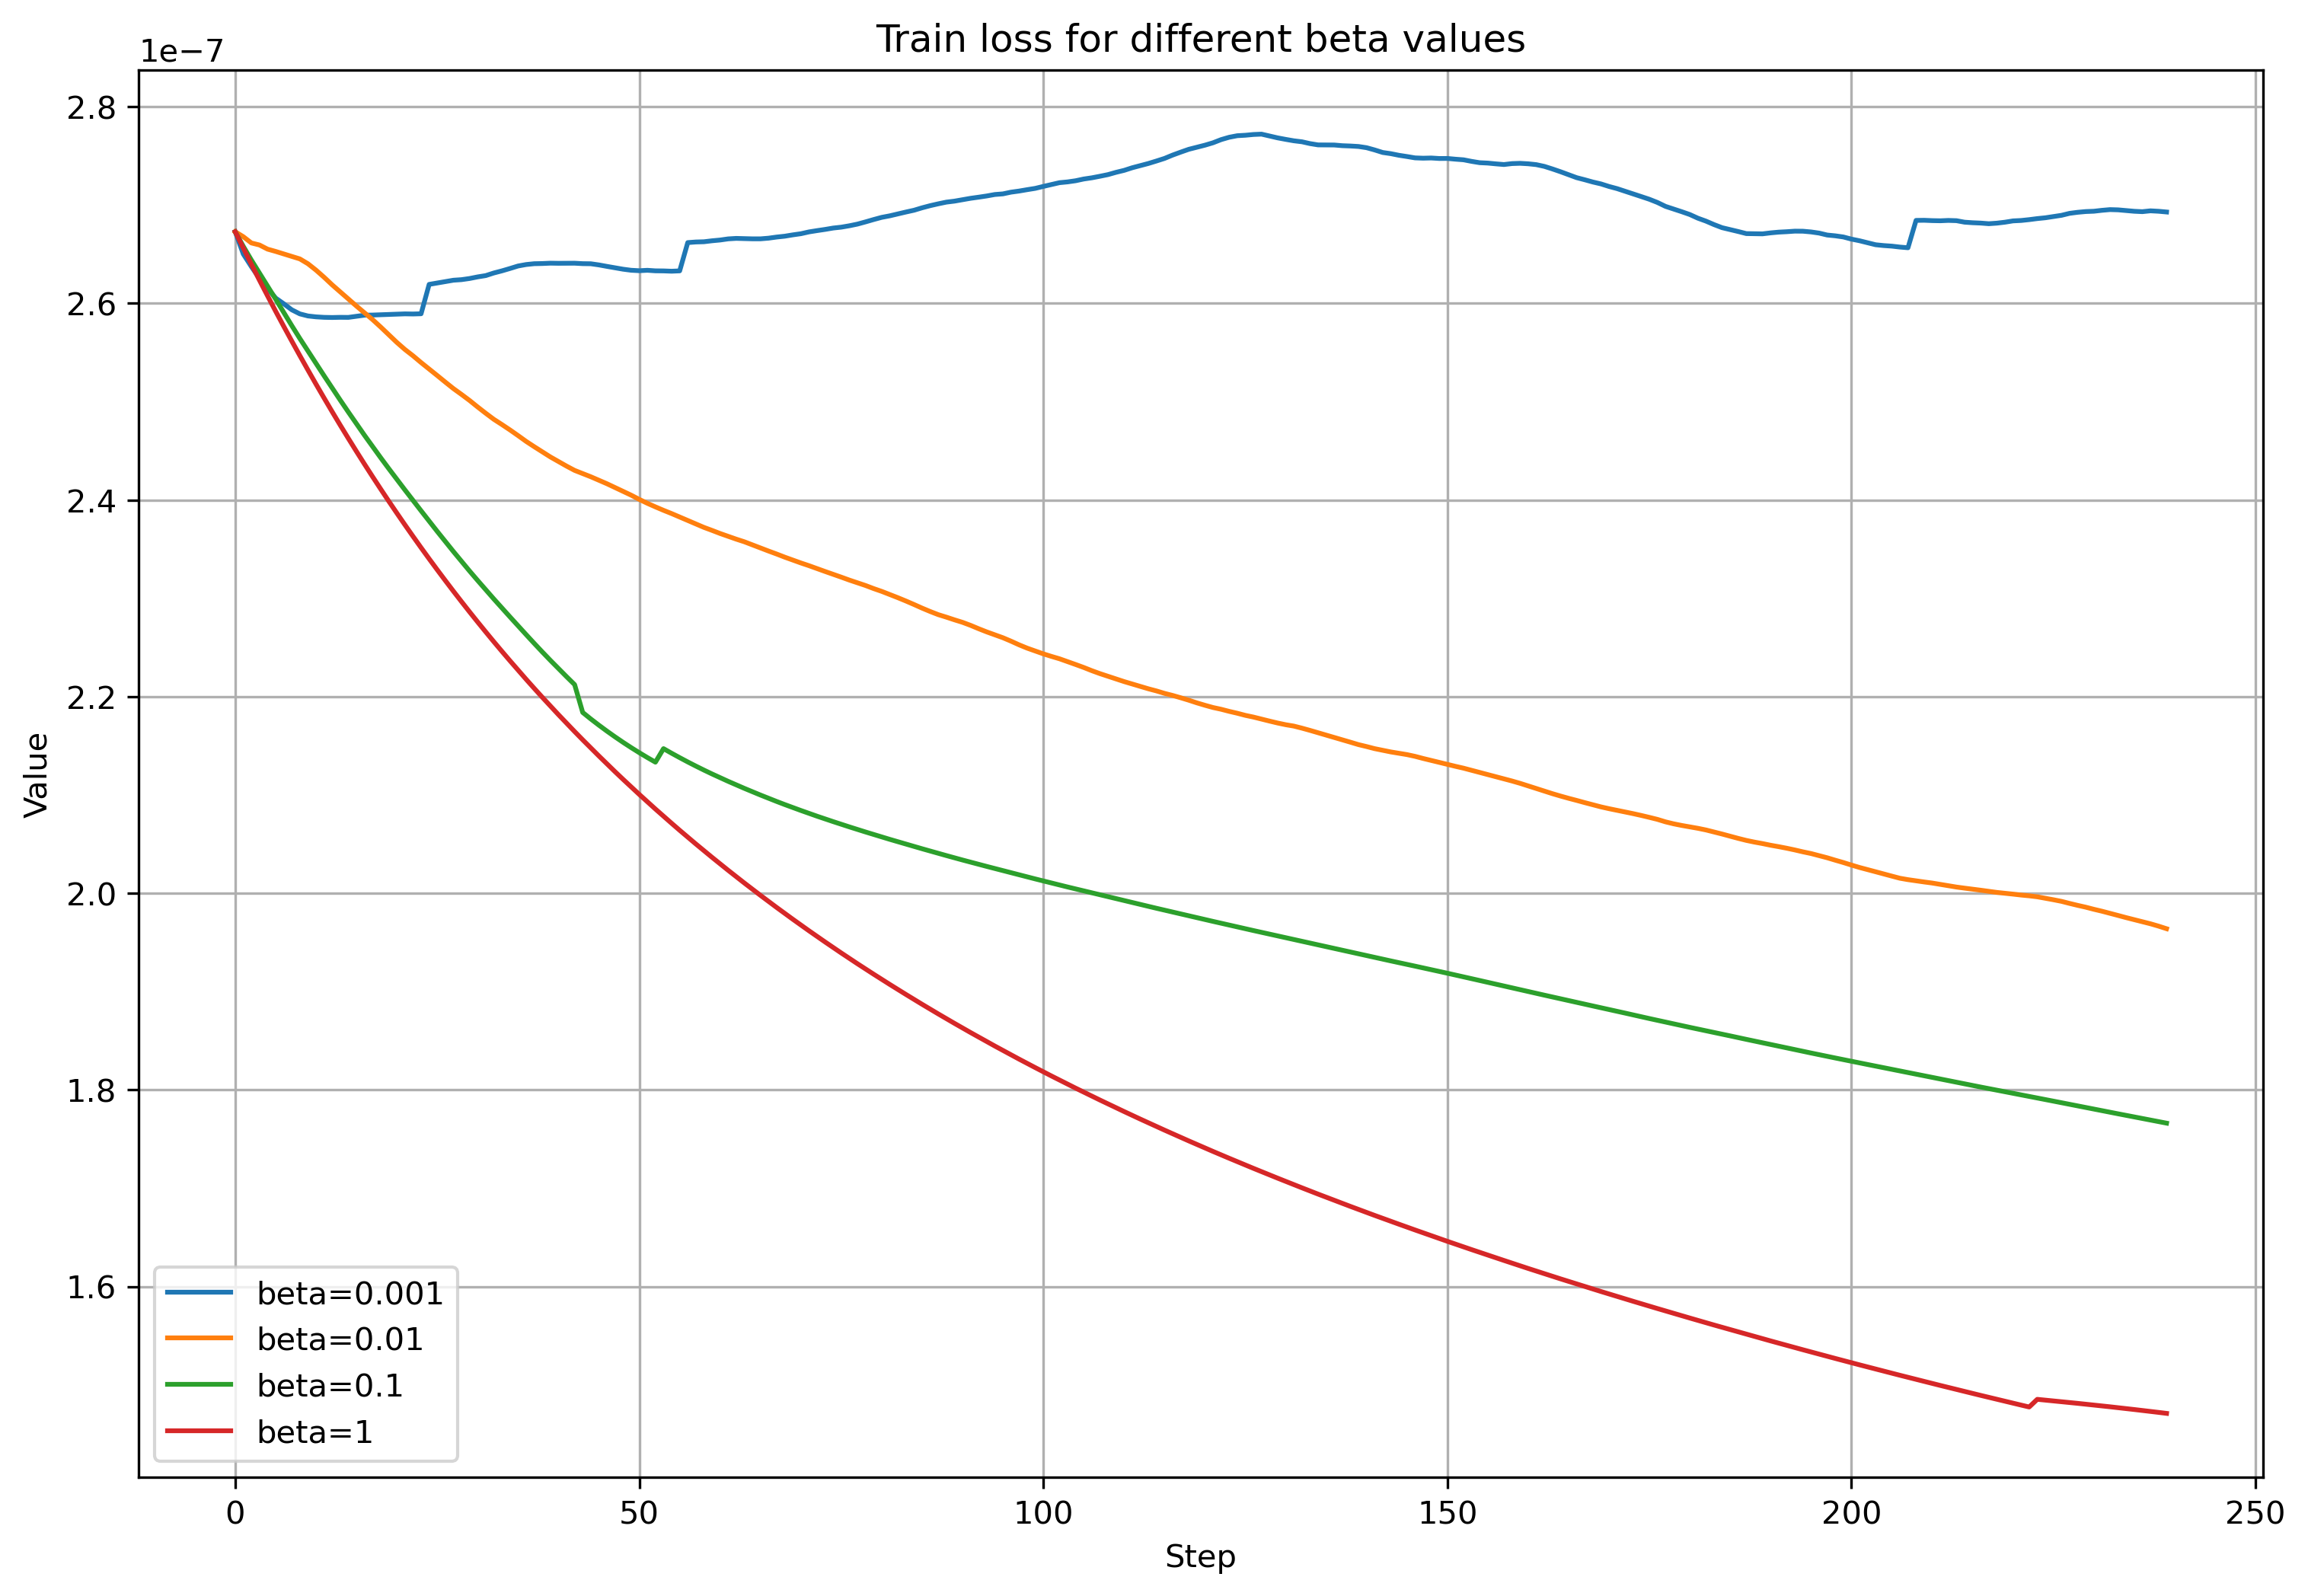
\includegraphics[scale=0.5]{images/train_loss_betas.png}
 \caption{Training loss for different valus of $\beta$ parameter.}
 % loss_comparison.png: 3002x2096 px, 300dpi, 25.42x17.75 cm, bb=0 0 720 50
 \label{fig:betas}
\end{figure}

\subsubsection{Summary of equilibrium propagation approach}
Equilibrium propagation proved to be more and applicable. I managed to decrease the implicit loss on one molecule, but more work needs to be done to make training on full dataset viable.
\section{Other results}

\subsection{Stability issues}
Implicit loss training falls under the framework of deep equilibrium model (DEQ). One of the issues plaguing DEQ models is training stability. As training goes on, obtaining the fixed point takes longer and longer. This is reported in \cite{opticalflow}, \cite{bai2021stabilizing}, \cite{burger2025dequify}, and \cite{geng2023torchdeq}. This was also the case for me when training multiple molecules; however, I did not encounter it when training on a single molecule. To alleviate the issue, I adapted a technique introduced in \cite{opticalflow} called \textbf{fixed point correction}. I am not aware of any explanation why the technique works. It stabilizes the training, although it can hurt performance; therefore, more work is required to make it suitable for fine-tuning.

Implementation and details of the fixed point correction technique are described in section \ref{sec:fpc}.

It would be beneficial to make the technique compatible with warm-starting, since that would allow for dramatic improvements in stability and training speed.

Figure \ref{fig:stability} shows a plot of the number of unconverged runs plotted against the total number of runs. The fixed point search parameters were chosen such that every molecule converged before fine-tuning.
\begin{figure}[H]
 \centering
 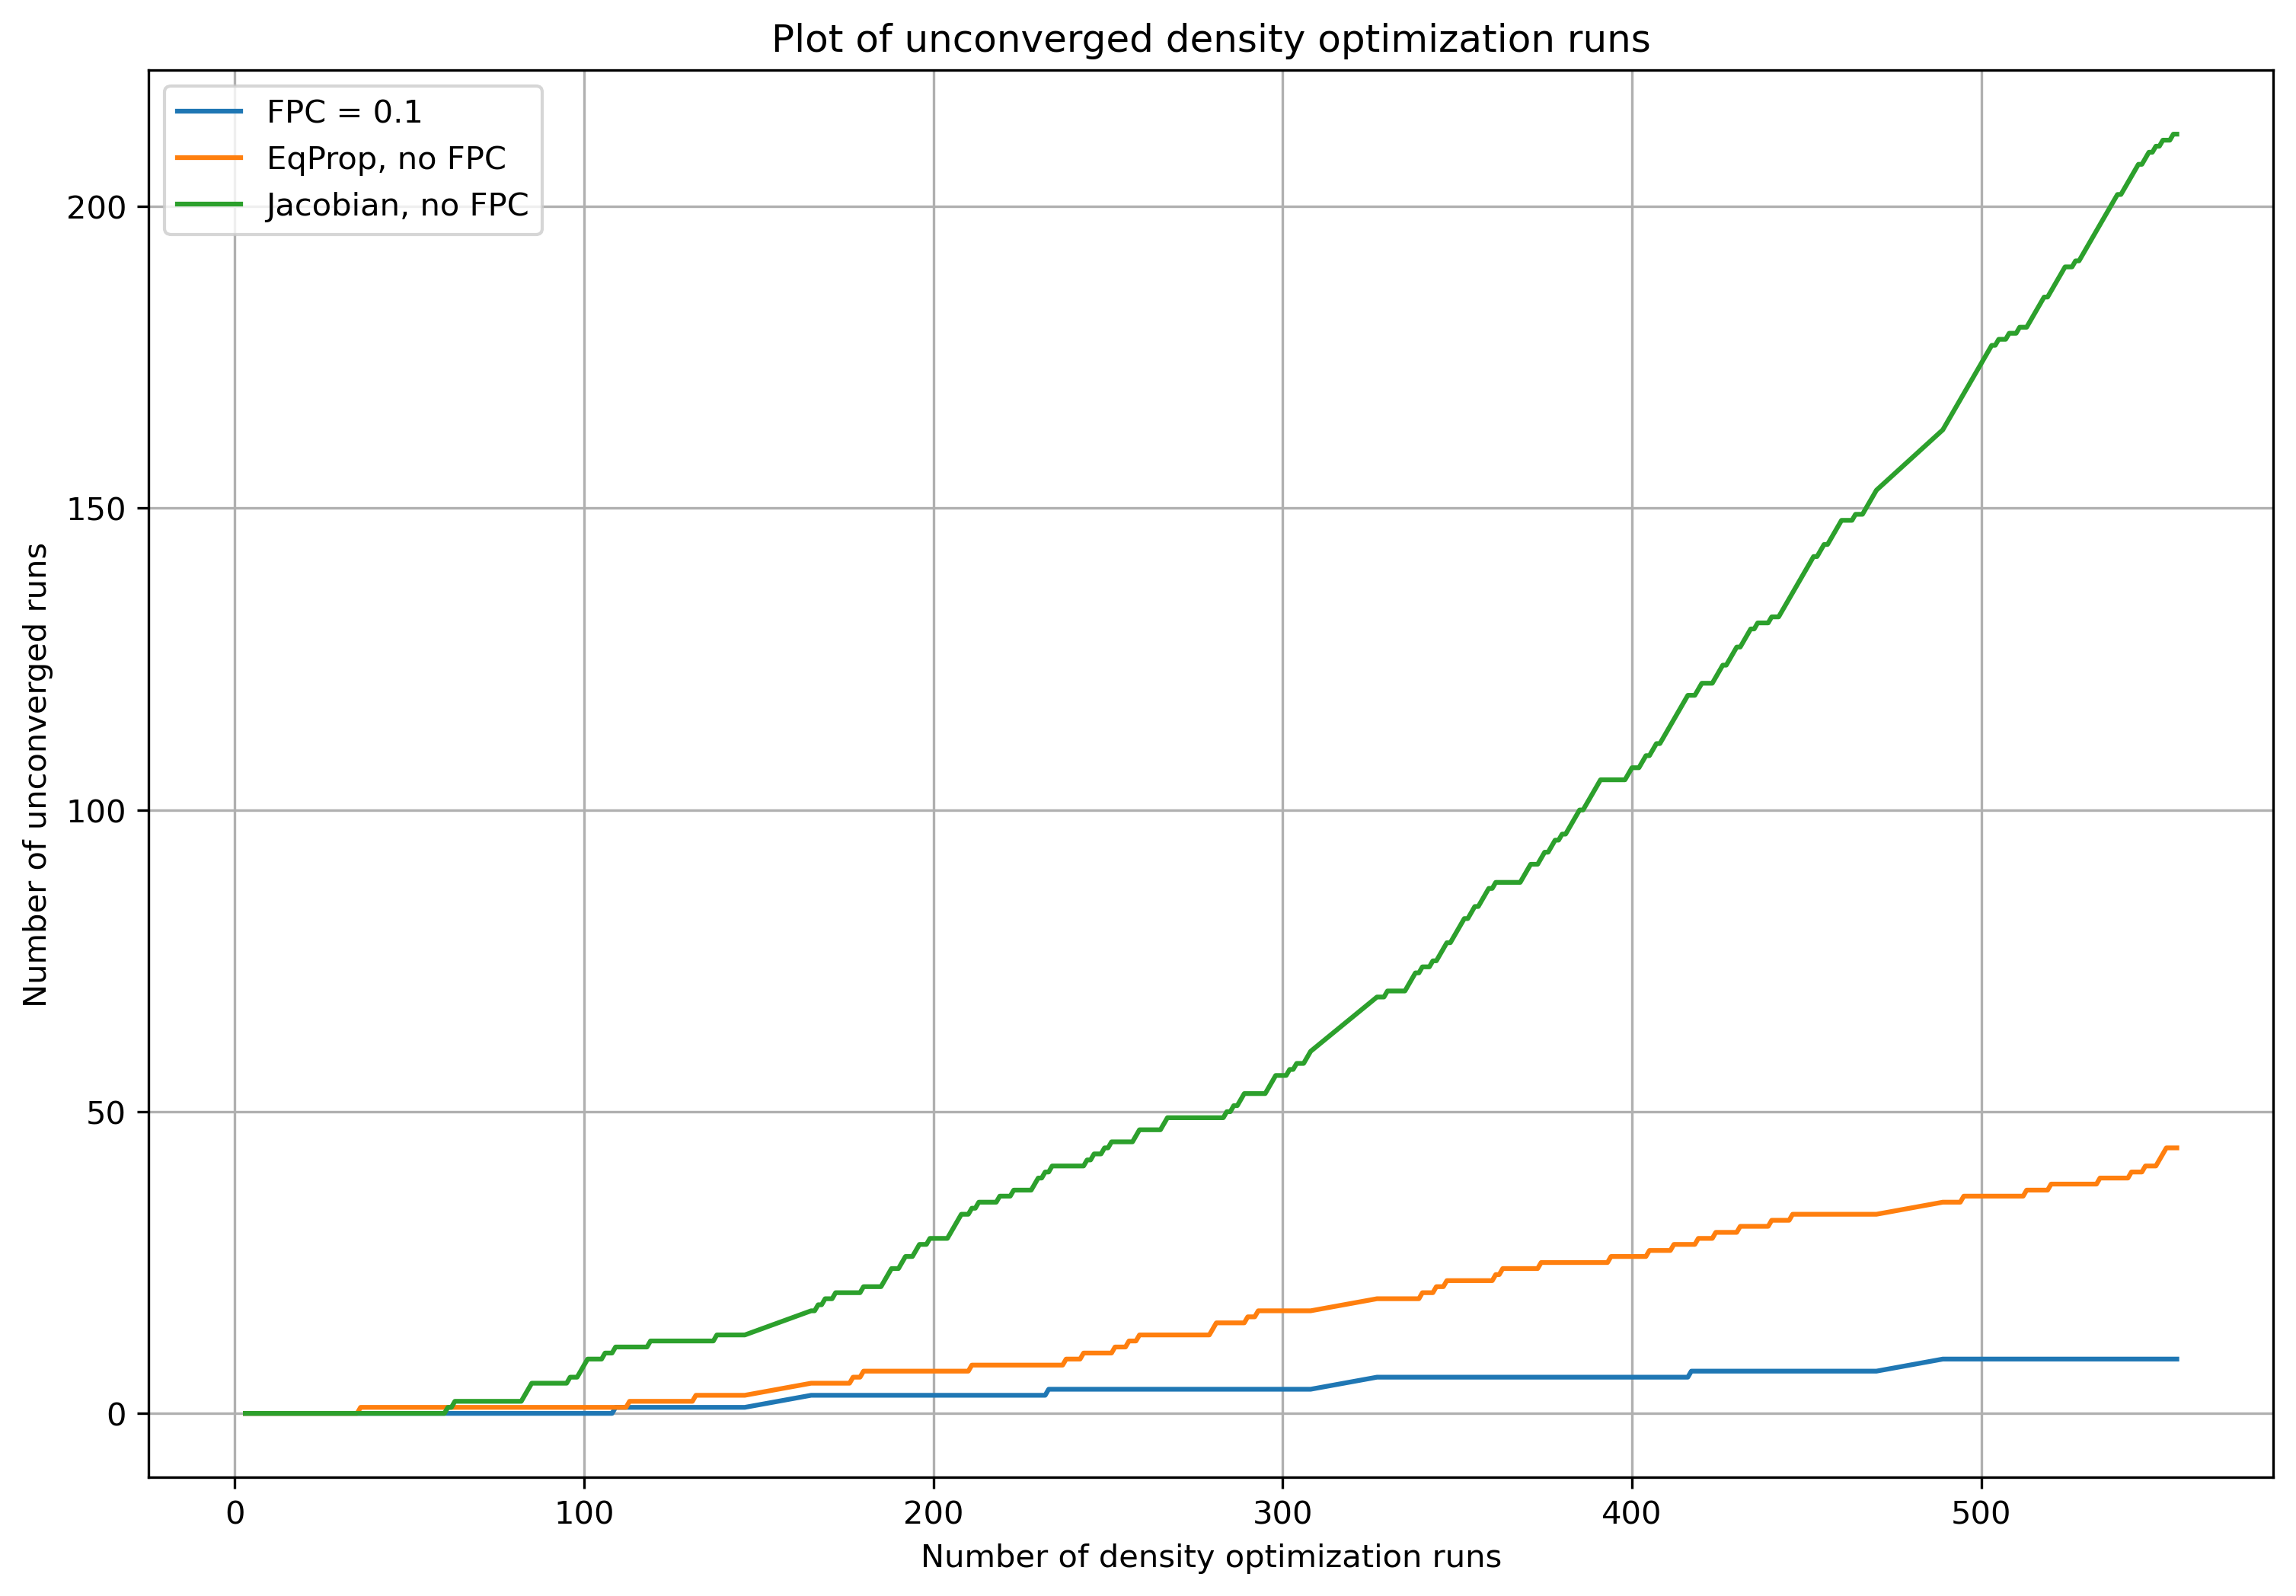
\includegraphics[scale=0.5]{images/stability_plot.png}
 \caption{Number of unconverged density optimization runs for EqProp approach with jacobian approach with no fixed point correction (top curve),no fixed point correction (middle curve) and  fixed point correction $=0.1$ (bottom curve).}
 % loss_comparison.png: 3002x2096 px, 300dpi, 25.42x17.75 cm, bb=0 0 720 50
 \label{fig:stability}
\end{figure}



\subsubsection{Training on more than one molecule}
After resolving stability issue I tested equilibrium propagation approach on a sample containing 180 and 1800 molecules taken from [name of the dataset, QMUGS or QM9]. I split the dataset in 80:10:10 ratios of train, validation and test, although test dataset ended up not being used. Regrettably, although train loss decreased, there was no improvement in validation loss and therefore no generalization.


\begin{remark}
 The problem \ref{bilevel} falls under \textbf{bilevel optimization}. However, due to memory and computational constraints the gradient is computed in mini-batches. It's possible, that \textbf{stochastic bilevel optimization} requires adaptation to make it work due to its nested structure or effect on variance of the gradient update.
\end{remark}

\clearpage
\section{Conclusions}
During the course of my internship at Hamprech Lab I have implemented and tested two approaches to implicit loss calculations. I have found that jacobian approach was not viable for the model I used and did not results in any metric improvement.
However equilibrium propagation approach did decrease targeted metrics. I have also encountered grevious model training stability issues and after extensive literature search adapted the technique to my setting.

Therefore, equilibrium propagation was shown to be an alternative method for optimizing losses defined implicitly, even when jacobian approach doesn't work.

On more personal level I learned working with version control within group, to conduct literature search, acquired knowledge about, TK how to do do experiments better.

Future directions:
TK make jacobian approach work
TK implement warm starting
TK resolve stability further
TK tracking loss function improvements for different molecules is quite hard
\nocite{*}
\bibliographystyle{plain}
\bibliography{references.bib}



\appendix
\section{Implementation details} \label{sec:impl}

\subsubsection{Model architecture}
I used a standard Graphormer model, which was trained on combination of QMUGS and QM9 datasets for $90$ epochs. The model architecture was based on the one in article \cite{zhang2024overcoming}.

\subsection{Fixed point search}
To obtain the fixed I used projected gradient descent with momentum with learning rate $\alpha = 5\cdot 10^{-3}$ and momentum $\beta = 0.9$. I ran the algorithm until gradient norm fell below tolerance threshold, which in most cases was set as $\epsilon = 10^{-4}$. The starting point was set to $p_{gs}$ and the maximum number of gradient descent steps was set to $100$.

\subsection{Fine-tuning on single molecule}
I trained the model with $Adam$ algorithm with learning rate equal to $10^{-7}$ and weight decay set to $0$ for $4$ epochs. Each epoch consisted of $80$ weight updates.
% \subsubsection{Gradient calculation}
% Gradients are obtained using automatic differentation
% The algorithm for finding fixed point is projected gradient descent. Its starting point was set to ground state $p_{gs}$.
% TK ADD threshold details
%
% Both vjp can be obtained efficiently using automatic differen in PyTorch, so naturally I preferred using matrix free methods.

\subsection{Fixed point correction}\label{sec:fpc}
Fixed point correction is a technique for stabilizing DEQ training. The technique is described in \cite{opticalflow}, \cite{geng2023torchdeq}
and \cite{burger2025dequify}. It is as follows.

Given fixed point trajectory $p_0= p_{gs}, p_1,\ldots, p_T\approx  \pth $ we uniformly select $N$ intermediate points $p_{i_1}, p_{i_2}, \ldots , p_{i_N}=p_T$ and compute the loss
\begin{equation}
 \mathcal{L}_{FPC}(\theta) = \sum_{k=1}^{n}\gamma^{n-k}\mathcal{L}(p_{i_k}),
\end{equation}
where gradient for each individual loss $\mathcal{L}(p_{i_k})$ is computed by treating as if $p_{i_k}$ was a fixed point. Typical value of $\gamma$ parameter is $0.8$ and it was also the one I used.
\par
I modified this technique in a stochastic way to account for varying number of fixed point steps for different molecules.

Let's fix $p\in (0,1)$. Then, for each point in fixed point trajectory, we decide select the intermediate point with probability $p$.
Finally, we compute the gradient based on the loss function
\begin{equation}
 \mathcal{L}_{FPC}(\theta) = \sum_{k=1}^{n}\gamma^{n-k+1}\mathcal{L}(p_{i_k}).
\end{equation}
\subsection{Linear equation}
TK solving yJ = b with vjp and jvp calls.

\end{document}
